\newpage
\chapter{Работа в основния прозорец}
\label{chapter02}

На различните операционни системи графичният потребителски интерфейс\index{потребителски интерфейс} изглежда по леко различен начин, но основните функционалности са едни и същи (Фиг. \ref{figure0007}).

\section{Основен работен екран}

\begin{figure}[h!]
  \centering
  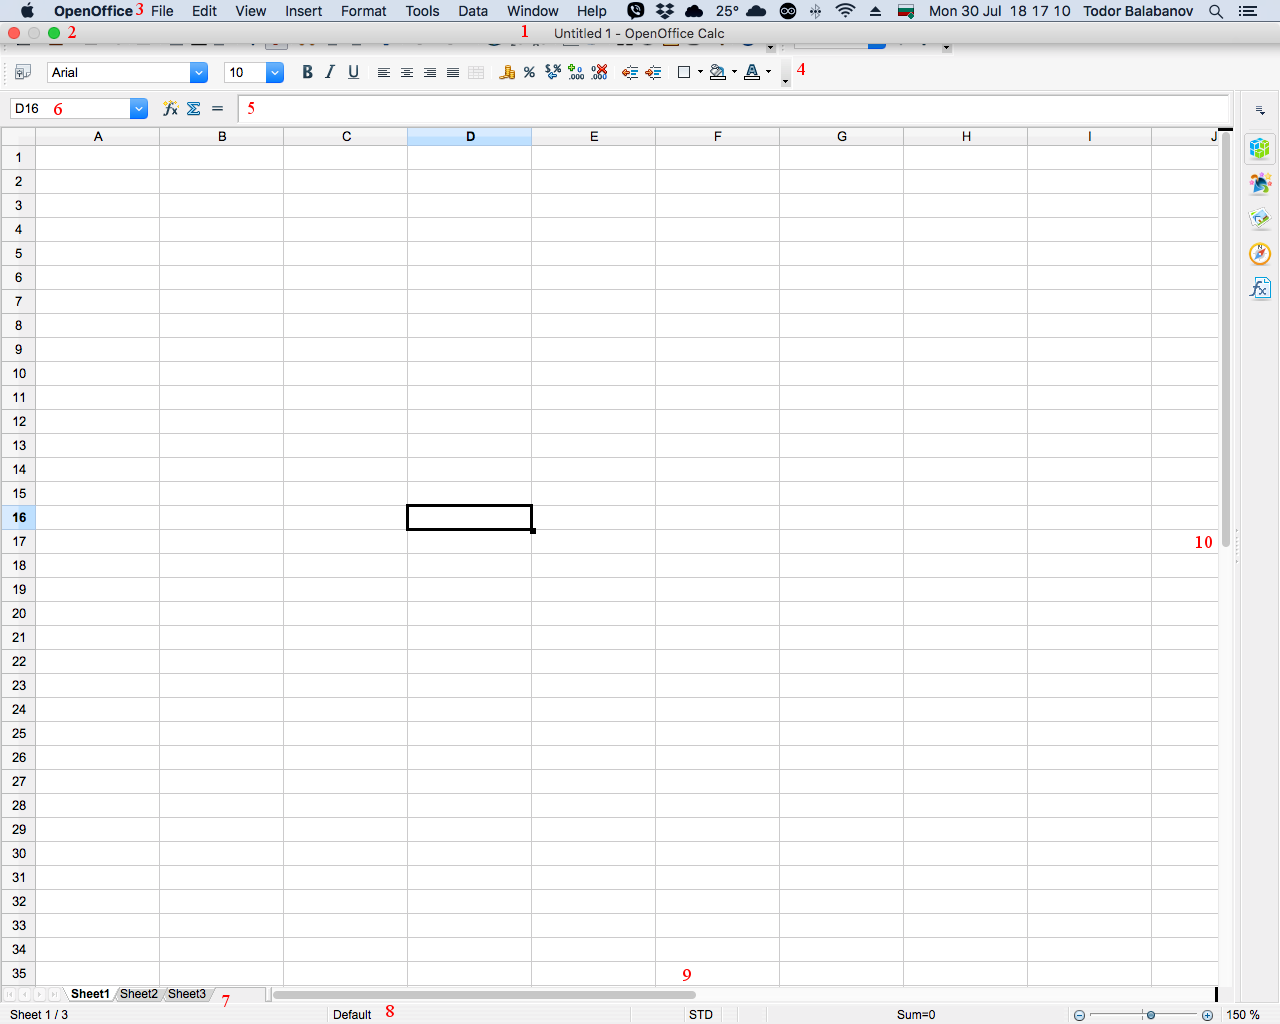
\includegraphics[width=1.0\linewidth]{pic0007}
  \caption{Заглавна лента с менюта}
\label{figure0007}
\end{figure}
\FloatBarrier

Най-отгоре (Фиг. \ref{figure0007} - 1), стои заглавната лента\index{заглавна лента} в която е изписано името на файла с който се работи. Когато не е зареден вече съществуващ файл, за име на файл се използва служебна комбинация от букви и цифри. В лявата част на заглавната лента се намират бутоните за управление на прозореца\index{управление на прозореца} (Фиг. \ref{figure0007} – 2). Над заглавната лента се намира лентата с менютата\index{лента с менюта} (Фиг. \ref{figure0007} – 3). На различните операционни системи лентата с менютата може да стои на различно място спрямо заглавната лента. Под заглавната лента стои панелът с инструментите (Фиг. \ref{figure0007} – 4). Под панела с инструментите стои панелът за въвеждане на формули\index{въвеждане на формули} (Фиг. \ref{figure0007} – 5). От ляво на панела за формули стои панела за въвеждане на адрес, за клетка или регион от клетки\index{адресиране на клетки} (Фиг. \ref{figure0007} – 6). Долу, в ляво са разположение работните листи\index{работни листи} (Фиг. \ref{figure0007} – 7). От дясно на работните листи се намира лентата за състоянието\index{лента на състоянието} на документа (Фиг. \ref{figure0007} – 8). Хоризонталният (Фиг. \ref{figure0007} – 9) и вертикалният (Фиг. \ref{figure0007} – 10) плъзгачи служат за преглеждане на работната област, когато тя надвишава видимата област от екрана. 

\section{Менюта}

